%preamble
\documentclass[letterpaper]{article}\usepackage[]{graphicx}\usepackage[]{color}
%% maxwidth is the original width if it is less than linewidth
%% otherwise use linewidth (to make sure the graphics do not exceed the margin)
\makeatletter
\def\maxwidth{ %
  \ifdim\Gin@nat@width>\linewidth
    \linewidth
  \else
    \Gin@nat@width
  \fi
}
\makeatother

\definecolor{fgcolor}{rgb}{0.345, 0.345, 0.345}
\newcommand{\hlnum}[1]{\textcolor[rgb]{0.686,0.059,0.569}{#1}}%
\newcommand{\hlstr}[1]{\textcolor[rgb]{0.192,0.494,0.8}{#1}}%
\newcommand{\hlcom}[1]{\textcolor[rgb]{0.678,0.584,0.686}{\textit{#1}}}%
\newcommand{\hlopt}[1]{\textcolor[rgb]{0,0,0}{#1}}%
\newcommand{\hlstd}[1]{\textcolor[rgb]{0.345,0.345,0.345}{#1}}%
\newcommand{\hlkwa}[1]{\textcolor[rgb]{0.161,0.373,0.58}{\textbf{#1}}}%
\newcommand{\hlkwb}[1]{\textcolor[rgb]{0.69,0.353,0.396}{#1}}%
\newcommand{\hlkwc}[1]{\textcolor[rgb]{0.333,0.667,0.333}{#1}}%
\newcommand{\hlkwd}[1]{\textcolor[rgb]{0.737,0.353,0.396}{\textbf{#1}}}%

\usepackage{framed}
\makeatletter
\newenvironment{kframe}{%
 \def\at@end@of@kframe{}%
 \ifinner\ifhmode%
  \def\at@end@of@kframe{\end{minipage}}%
  \begin{minipage}{\columnwidth}%
 \fi\fi%
 \def\FrameCommand##1{\hskip\@totalleftmargin \hskip-\fboxsep
 \colorbox{shadecolor}{##1}\hskip-\fboxsep
     % There is no \\@totalrightmargin, so:
     \hskip-\linewidth \hskip-\@totalleftmargin \hskip\columnwidth}%
 \MakeFramed {\advance\hsize-\width
   \@totalleftmargin\z@ \linewidth\hsize
   \@setminipage}}%
 {\par\unskip\endMakeFramed%
 \at@end@of@kframe}
\makeatother

\definecolor{shadecolor}{rgb}{.97, .97, .97}
\definecolor{messagecolor}{rgb}{0, 0, 0}
\definecolor{warningcolor}{rgb}{1, 0, 1}
\definecolor{errorcolor}{rgb}{1, 0, 0}
\newenvironment{knitrout}{}{} % an empty environment to be redefined in TeX

\usepackage{alltt}
\usepackage[OT1]{fontenc}
\usepackage{fullpage} %the fullpage.sty file needs to be copied somewhere
                    %into the MiKTeK search path. 
\usepackage{tabularx} % for getting wide tables to fit properly
\usepackage{enumerate} % for alphanumeric lists with {enumerate}[(A)]
\usepackage{amsmath} % for access to {equation*} and {aligned} functions for equations
\usepackage{subfigure} %create multi-part figures
\usepackage{setspace} %package for setting line spacing
\usepackage{framed} % for making boxes around Tex text
\usepackage{cclicenses} % for creative commons logos
%\usepackage{draftwatermark} % for adding water mark over instructor version
% Use siunitx package for proper upright greek letters in text, \umol = ?mol
% give package arguments in [] brackets, then give package name in {} brackets
\usepackage[free-standing-units=true,
            space-before-unit=true,
            use-xspace=true]{siunitx} 
%\usepackage{gensymb}
\usepackage{float} % Get access to [H] argument for figure placement
\usepackage{fancyhdr} %for making fancy headers/footers
\pagestyle{fancy} %required for fancy headers
\usepackage{lastpage} % used for showing page X of pages XX in footer
\usepackage{soul} % access to the \hl yellow high-light command
% get access to \definecolor and \textcolor{} \cellcolor{} for coloring text
% in the text and tables
\usepackage[usenames,dvipsnames,table]{xcolor}
\definecolor{webred}{rgb}{0.7, 0, 0} % less intense red color
\definecolor{webblue}{rgb}{0, 0, 0.7} % less intense blue color 
% Use the hyperref package below to create bookmarks in the output pdf. This 
% will convert numbered sections into bookmarks, and will link figure/table 
% references in the text to their respective captions. Also enables the \url{} 
% and \href{} functions. Load this as the last package in the preamble, unless
% you also use \usepackage[all]{hypcap} to display figures from hyperlinks more
% naturally, in which case hypcap should be the last package loaded.
\usepackage[pdftex, 
            bookmarks=true, 
            bookmarksnumbered=true,
            bookmarksopen=true,
            colorlinks=true,
            linkcolor=webred,
            urlcolor=webblue]{hyperref}
\usepackage[all]{hypcap} % include after hyperref package

\setstretch{1.2}    %set line spacing.
\newcommand\T{\rule{0pt}{2.6ex}} %used for padding table cells vertically
\newcommand\B{\rule[-1.2ex]{0pt}{0pt}} %used for padding table cells vertically
%%%%%%%%%%%%%%%%%%%%%%%%%%%%%%%%%%%%%%%%%%%%%%%%%%%%%%%%%%%%%%%%%%%%%%%%%%%%%%%%%%%%%
%%%%%%%%%%%%%%%%%%%%%%%%%%%%%%%%%%%%%%%%%%%%%%%%%%%%%%%%%%%%%%%%%%%%%%%%%%%%%%%%%%%%%
% Set some knitr options


%%%%%%%%%%%%%%%%%%%%%%%%%%%%%%%%%%%%%%%%%
% Change the value of showInstruct below to switch from student to instructor
% version of the document


%%%%%%%%%%%%%%%%%%%%%%%%%%%%%%%%%%%%%%%%%%%%%%%%%%%%%%%%%%%%%%%%%%%%%%%%%%%%%%%%
%%%%%%%%%%%%%%%%%%%%%%%%%%%%%%%%%%%%%%%%%%%%%%%%%%%%%%%%%%%%%%%%%%%%%%%%%%%%%%%%
\title{\vspace{-2.0cm}A test document}
\author{}
\date{}
\IfFileExists{upquote.sty}{\usepackage{upquote}}{}
\begin{document}
%%%%%%%%%%%%%%%%%%%%%%%%%%%%%%%%%%%%%%%%%%%%%%%%%%%%%%%%%%%%%%%%%%%%%%%%%%%%%%%
% define header/footer
% This is mostly window dressing, but I use it as an opportunity to stick
% a marker for the student/instructor version of the document in the footer
\pagestyle{fancy}
\headsep = 5 pt
\headwidth = \textwidth
\lhead{}
\chead{}
\rhead{}
\lfoot{}
\cfoot{Student version}

%\cfoot{} 
\rfoot{Page \thepage~of \pageref{LastPage}}
\renewcommand{\headrulewidth}{0.0pt}
\renewcommand{\footrulewidth}{0.4pt}
%finished defining header/footer
%%%%%%%%%%%%%%%%%%%%%%%%%%%%%%%%%%%%%%%%%%%%%%%%%%%%%%%%%%%%%%%%%%%%%%%%%%%%%%%
\maketitle
\vspace{-1.0cm}



\pagenumbering{arabic}  % start regular arabic page numbers
%%%%%%%%%%%%%%%%%%%%%%%%%%%%%%%%%%%%%%%%%%%%%%%%%%%%%%%%%%%%%%%%%%%%%%%%%%%%%%%

\section{Always-visible code}
Let's pretend we're writing a real lab handout. We'd start with some example
code that the students might want run, but the code shown here wouldn't 
actually work as written.

\begin{knitrout}
\definecolor{shadecolor}{rgb}{0.969, 0.969, 0.969}\color{fgcolor}\begin{kframe}
\begin{alltt}
\hlcom{# This would cause an error if actually executed}
model = \hlkwd{lm}( your dummy ~ formula here, data = your data frame) 
\end{alltt}
\end{kframe}
\end{knitrout}

But here's some code that does execute properly, because both of the chunk 
options \texttt{echo} and \texttt{eval} are \texttt{TRUE}:

\begin{knitrout}
\definecolor{shadecolor}{rgb}{0.969, 0.969, 0.969}\color{fgcolor}\begin{kframe}
\begin{alltt}
\hlcom{# Generate some data}
\hlstd{x} \hlkwb{=} \hlkwd{seq}\hlstd{(}\hlnum{1}\hlstd{,}\hlnum{10}\hlstd{)}
\hlstd{y} \hlkwb{=} \hlstd{x} \hlopt{*} \hlnum{3} \hlopt{+} \hlkwd{rnorm}\hlstd{(}\hlnum{10}\hlstd{,}\hlnum{3}\hlstd{,}\hlnum{2}\hlstd{)}
\hlcom{# Run a correlation test}
\hlkwd{cor.test}\hlstd{(x,y)}
\end{alltt}
\begin{verbatim}
## 
## 	Pearson's product-moment correlation
## 
## data:  x and y
## t = 14.789, df = 8, p-value = 4.3e-07
## alternative hypothesis: true correlation is not equal to 0
## 95 percent confidence interval:
##  0.9239779 0.9959263
## sample estimates:
##       cor 
## 0.9821992
\end{verbatim}
\end{kframe}
\end{knitrout}

By default, \textsf{knitr} adds two hashmarks ahead of the output that is 
returned by R, as seen above for the output of the correlation test. 

%%%%%%%%%%%%%%%%%%%%%%%%%%%%%%%%%
\section{Hiding instructor code}
Next we'll write some R chunks that only show up when 
\texttt{showInstruct=TRUE}. If this is the instructor version, you should see
some R code to generate more data and another correlation test. But if this
is the student version, there should be no R code immediately below this line
in the PDF document.



If the instructor code was activated, you should have seen a chunk of R 
output above this line in the PDF document. 

\begin{framed}
\textbf{Exercise:} In the student version, this boxed section would contain a 
question to be answered. 

\end{framed}

We can also include some regular text that will only appear in the 
instructor version. A box with text should appear below in the PDF document
if the instructor version is active, but in the student version the next section 
will start instead. 



%%%%%%%%%%%%%%%%%%%%%%%
\section{Figures}

Including a figure in the student and instructor version is fairly 
straightforward if you're used to writing TeX code.

\begin{knitrout}
\definecolor{shadecolor}{rgb}{0.969, 0.969, 0.969}\color{fgcolor}\begin{kframe}
\begin{alltt}
\hlkwd{plot}\hlstd{(x,y,} \hlkwc{type} \hlstd{=} \hlstr{'b'}\hlstd{,} \hlkwc{las} \hlstd{=} \hlnum{1}\hlstd{,} \hlkwc{main}\hlstd{=}\hlstr{'Student version'}\hlstd{)}
\end{alltt}
\end{kframe}
\end{knitrout}
% Insert the figure using the code below. Currently knitr is appending
% a -1 to all my figure names, so I have to include that when I reference 
% the figure in the \includegraphics call below
\begin{figure}[H]
\centering
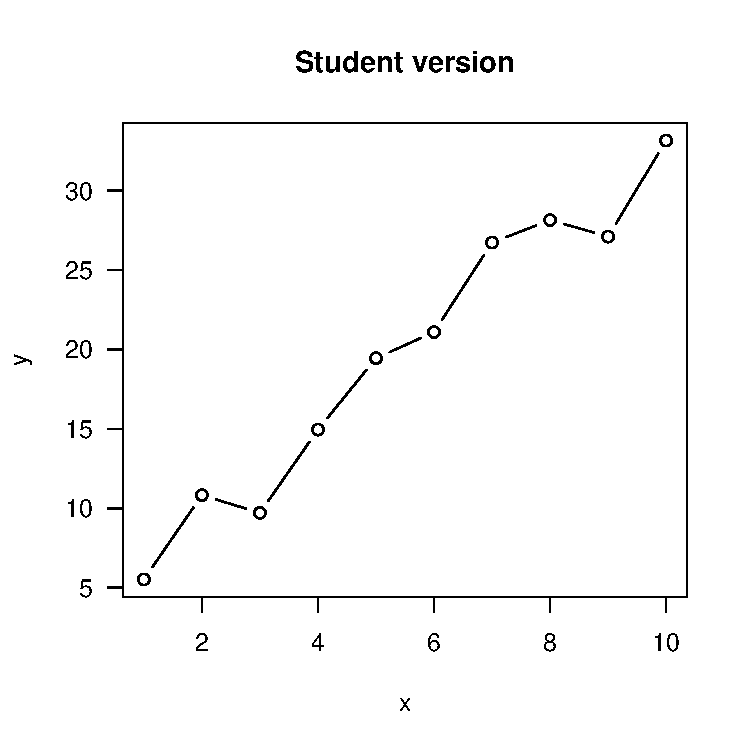
\includegraphics[width=0.5\textwidth]{figs/studentPlot-1}
\caption{A simple plot, included by default in both student and instructor
versions of the handout.}
\label{fig:studentPlot}
\end{figure}

Next we'll try the instructor-only plotting. A figure should only show up
when you have set \texttt{showInstruct=TRUE} up near the start of the .Rnw
document (line 63 on this file). But if this is the student version, there will 
be nothing after this line. 






%%%%%%%%%%%%%%%%%%%%
\end{document}
